\section{Logistic Regression}
Hier geht es um Daten die Binär klassifiziert werden (Ja-Nein Fragen). Beispiel: Wird es Hageln aufgrund eines Satellitenbilds. Oder hat jemand bald ein Epsilepsie-Anfall wegen einem EEG reading. \\
\\
In solchen Fällen sehen die Daten anderst aus, weshalb wir ein anderes Modell und Loss-Funktion brauchen. (Lineare Funktion geht nicht) Für den Optimizer können wir aber weiterhin Gradient Descent verwenden, da die andere Loss-Funktion convex ist.
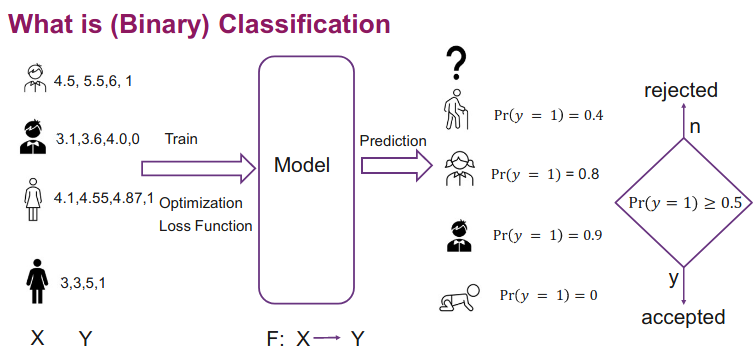
\includegraphics[width=\linewidth]{img/binary_classification.png}
\subsection{Warum nicht Lineares Modell?}
Das Problem der Linearen Regression ist, dass die Kurve ganz anders aussieht, sobald ein weiterer Datensatz dazu kommt und Tresholding hier falsche Ergebnisse liefern kann. Die Kostenfunktion (Loss) Min Squared Error funktioniert hier gar nicht und liefert diese falschen, verzerrten Ergebnisse. Wir sind aber interessiert in eine Warscheinlichkeits-Output. Somit brauchen wir ein Modell, dass die Wahrscheinlichkeit abbildet.
\subsection{Sigmoid Funktion}
Die Lösung ist die Sigmoid-Funktion. Sie bietet genau das benötigte Modell:
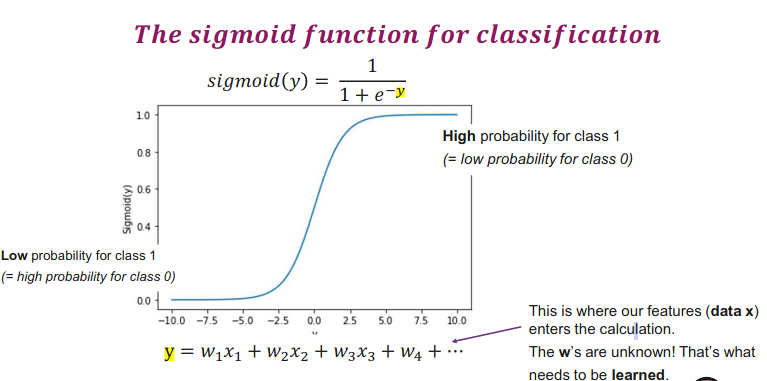
\includegraphics[width=\linewidth]{img/sigmoid.png}
Das y bzw. manchmal auch z kann alle Dimensionen enthalten. z.B.
$$y = w_1x_1=w_2x_2+w_3x_3+...$$
\subsection{Wahrscheinlichkeit}
Wir können die geschätze Wahrscheinlichkeit so schreiben:
$$Pr(y=1|x;W) = Pr(y=1 | x) = p(x) = \frac{1}{1+e^{-(W^Tx)}}$$
Für eine Vorhersage können wir schreiben $ p(x) = \frac{1}{1+e^{-(W^Tx)}}$ wobei man beachten sollte, dass p eine Zahl zwischen 0 und 1 ist.\\
\textbf{Wir haben nun das Modell aber wie bekommen wir W?}
\subsection{Maximum Likelyhood (Loss)}
Wenn man alle Datenpunkte (X, Y) hat, wollen wir die Wahrscheinlichkeit maximieren, dass alle Vorhersagen richtig sind (oder die Wahrscheinlichkeit minimieren, dass alle Vorhersagen falsch sind)!
Das Ziel des Trainings ist die Festlegung der Koeffizienten W so einzustellen, dass p nahe bei 1 liegt, wenn y = 1 und W nahe bei 0 liegt, wenn y = 0
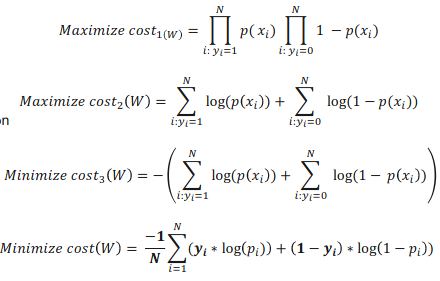
\includegraphics[width=\linewidth]{img/maximum_likelyhood.png}
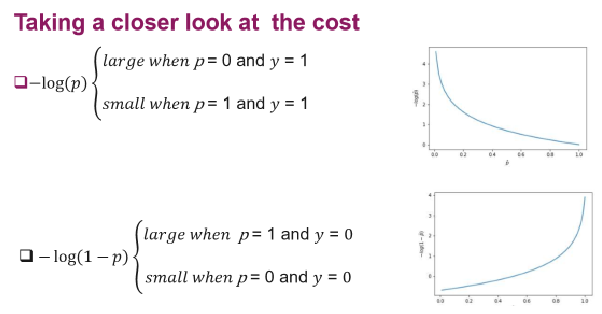
\includegraphics[width=\linewidth]{img/maximum_likelyhood_cost.png}